
\chapter{Field Tests}\label{ch:field_test}

Computer Vision algorithms can only give as good result as the source videostream that it is 
being fed. After talking a bit to \gls{sintef}, some test videos were provided by them. However, as seen in figure 
\vref{fig:sintef_not_1}, the quality leaves much to be desired. The video provided had a resolution 
of $854 \times 480$ pixels with big black box padding around it. This does not only make 
the video unsuitable for us in a computer vision algorithm, but it also means that the video 
probably is upscaled quite a bit.

Due to the poor nature of the quality of the video it was decided early on that 
a field test was needed, since we were going to use equivalent hardware as to what is available on the \gls{rov}. 

\begin{figure}[htbp]
	\centering
	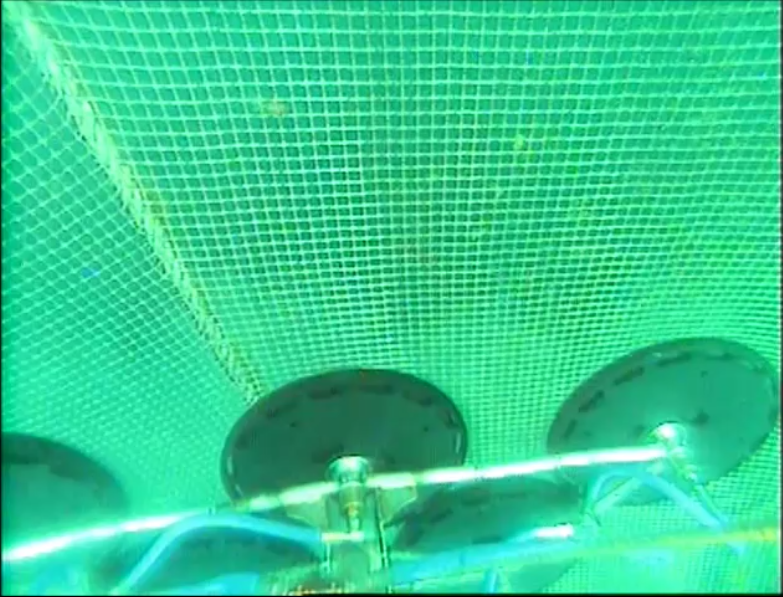
\includegraphics[width=\textwidth]{sintef_not_video_1}
	\caption{Original video provided by \gls{sintef}}
	\label{fig:sintef_not_1}
\end{figure}

\section{SINTEF DVL Test}\label{sec:sintef.test}
As part of the cooperation with \gls{sintef} during the preliminary testing, we 
were asked to help with a \gls{dvl} test using a rig for controlling 
the movement of the net. As a favour for us helping out, we 
got to lend the rig at a later time when our hardware were ready to do a field test. 

During this test, we learned enough about the rig and operation of it that we should be able to operate 
it ourselves. The field test also gave some valuable information 
on how to get everything set up correctly, and what preparations which 
were needed to go through with our test.

\begin{figure}[htbp]
	\centering
	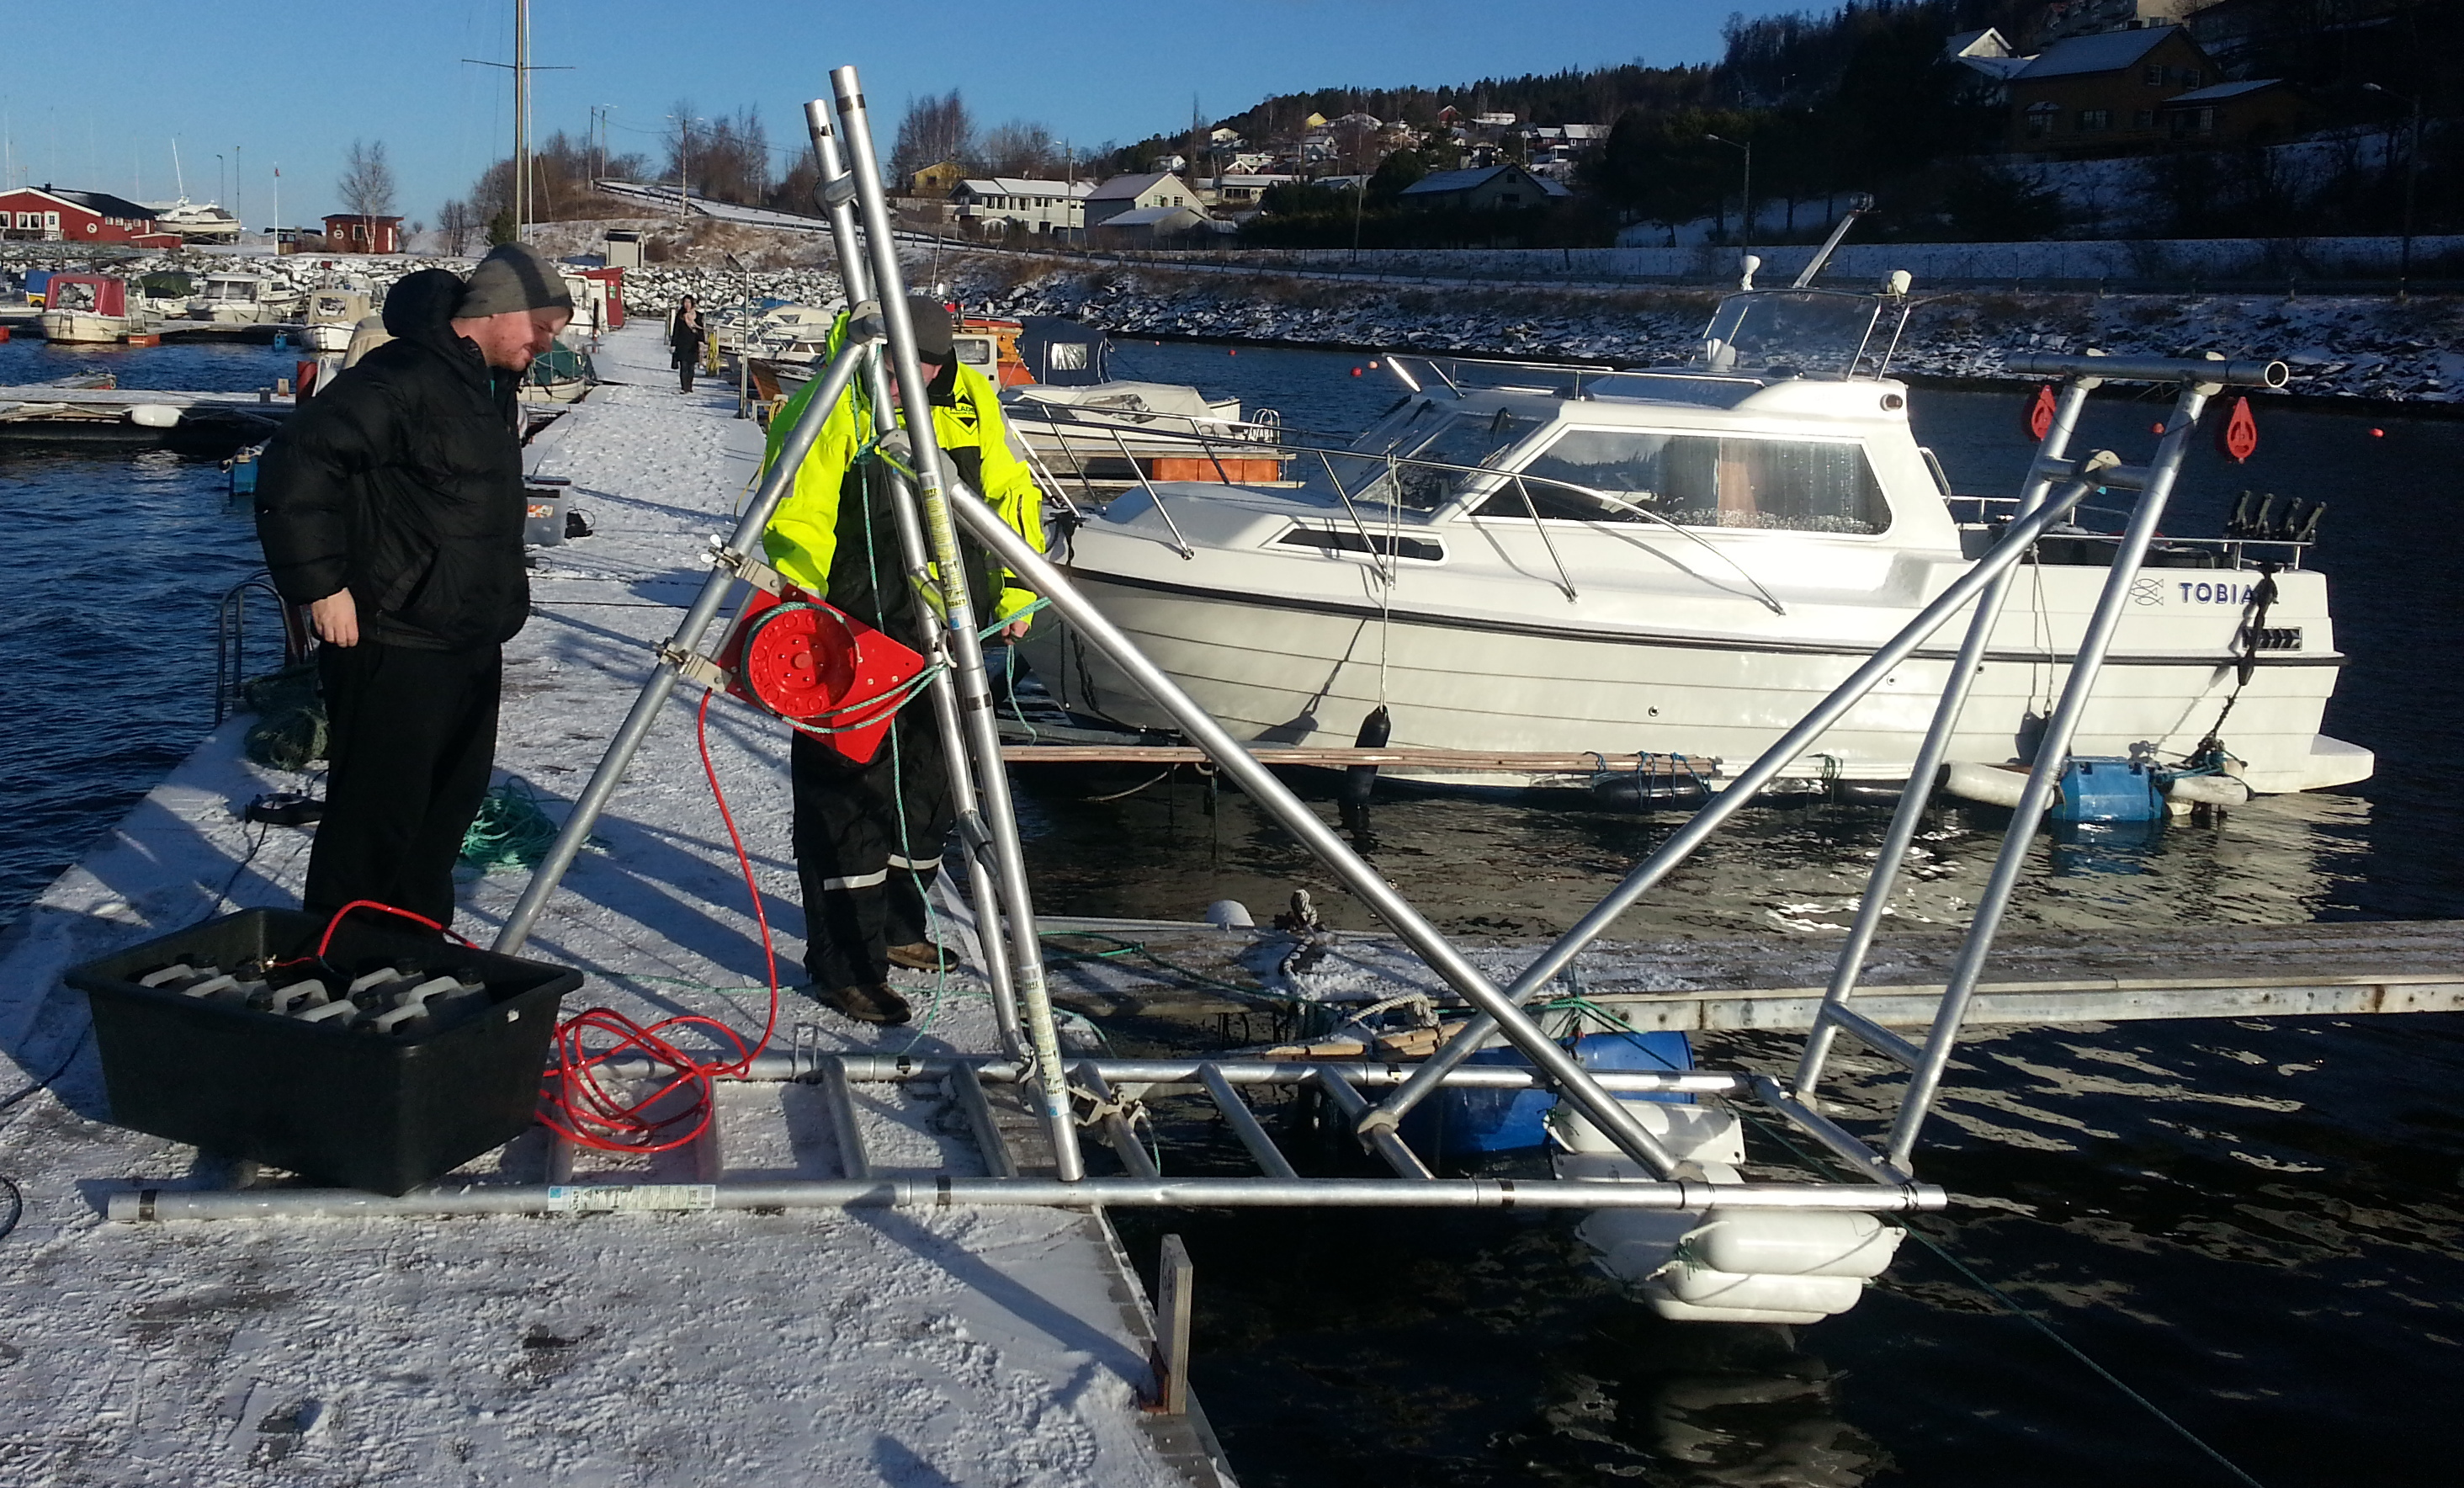
\includegraphics[width=\textwidth]{rig1}
	\caption{Field test for \gls{sintef} using \gls{dvl}}
	\label{fig:test_dvl}
\end{figure}

\section{HD Video Test}

\begin{table}[htbp]
	\centering
	\begin{tabular}{ll}
		\toprule
			Net setup 					& Description  \\
		\midrule
			Reference					& Net in static position. No forced movement. \\
			Reference with movement		& Net lowered in front of the camera. \\
			Circular hole				& Net with a circular cut-out lowered. \\
			Vertical tear				& Net with a narrow vertical tear lowered. \\
			Horizontal tear				& Net with narrow horizontal tear lowered. \\
			L-shaped tear				& Net with horizontal L-shaped tear lowered. \\
			Growth						& Net with imitation growths lowered.\\
			Double sea-cage				& Two nets laid on top of each other.\\
		\bottomrule
	\end{tabular}
	\caption{Test setup, all at \SI{1.5}{\metre}}
	\label{tbl:test_setup}
\end{table}

\begin{figure}[htbp]
    \centering
    \subfloat[Circular Hole]{\label{fig:net_hole}{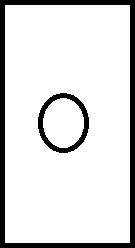
\includegraphics[width=0.3\textwidth]{net_hole}}} \hfill
    \subfloat[Vertical tear]{\label{fig:net_vertical}{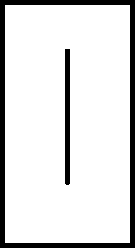
\includegraphics[width=0.3\textwidth]{net_vertical}}} \hfill
    \subfloat[Double net]{\label{fig:net_double}{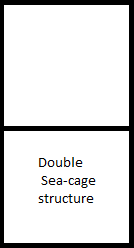
\includegraphics[width=0.3\textwidth]{net_double}}}
    \\
	\subfloat[L-shaped tear]{\label{fig:net_L_tear}{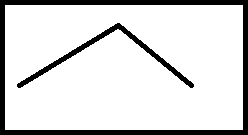
\includegraphics[width=0.45\textwidth]{net_l}}} \hfill
	\subfloat[Horizontal tear]{\label{fig:net_horize}{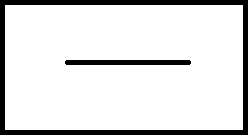
\includegraphics[width=0.45\textwidth]{net_horiz}}}
	\caption{Different net configurations with holes and tears, excluding normal single net. Images collected from \citet{sletta13}.}
	\label{fig:net_configs}
\end{figure}

\begin{figure}[htbp]
	\centering
	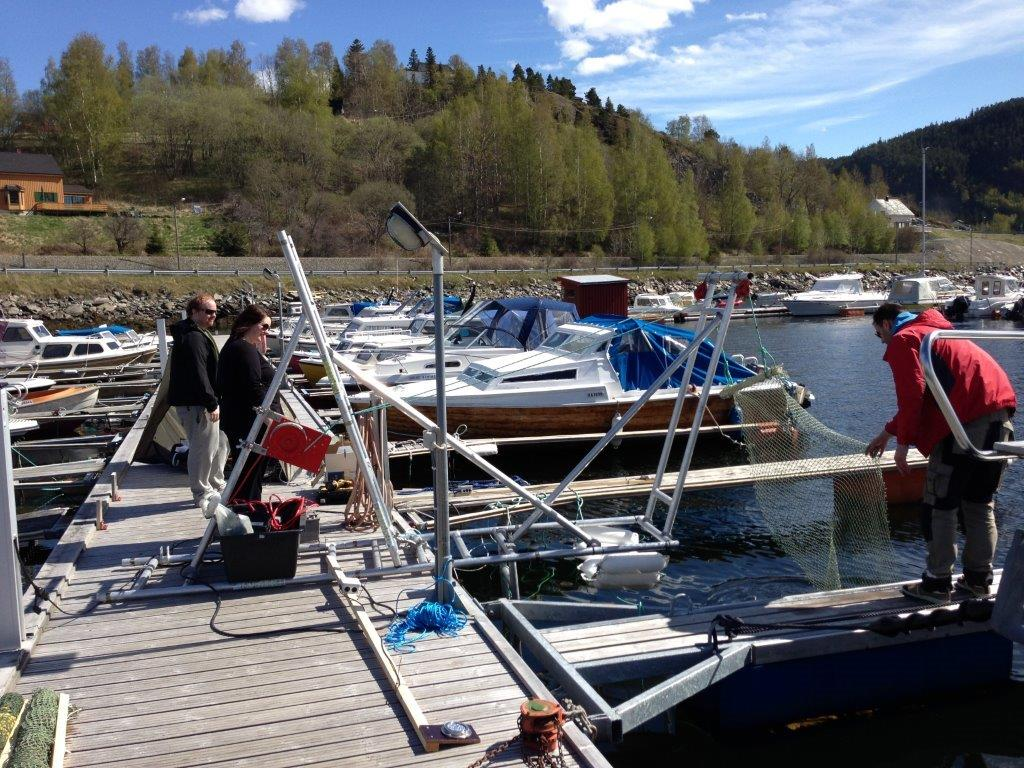
\includegraphics[width=0.9\textwidth]{rig2}
	\caption{Field test on a sunny day in May}
	\label{fig:test_hd}
\end{figure}

The rig was configured to mimic the approximate distance to the net 
in figure \vref{fig:sintef_not_1}. We were however not able to tilt the camera to 
an angle due to environmental constraint in a anchor chain situated below the camera.
We approximated the distance between the ROV and the net in figure \vref{fig:sintef_not_1} to be 
\SI{1.5}{\metre}. This lead to a the image in figure \vref{fig:test_hd_referanse}.

\begin{figure}[htbp]
	\centering
	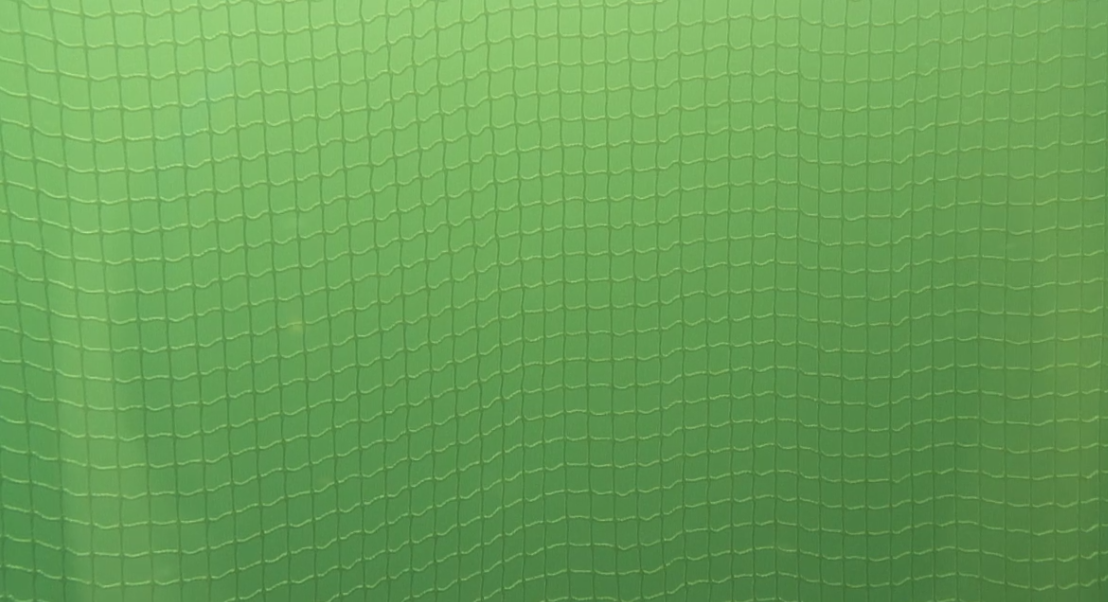
\includegraphics[width=\textwidth]{hd_not_all}
	\caption{View of the net from \SI{1.5}{\metre}. This is the default distance for the rig used.}
	\label{fig:test_hd_referanse}
\end{figure}

Comparing image \vref{fig:test_hd_referanse} and \vref{fig:sintef_not_1}, it seems that the 
top row of masks is approximately the same in both images. Due to the tilt of the 
camera in image \ref{fig:sintef_not_1} we get a prominent vanishing point in that image. There 
are also some growing on the net in figure \ref{fig:sintef_not_1}, which of obvious reasons does not appear 
in figure \ref{fig:test_hd_referanse}.

\begin{figure}[htbp]
	\centering
	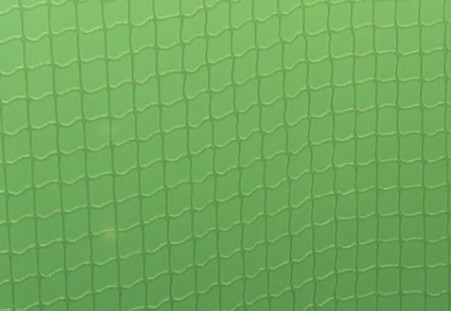
\includegraphics[width=\textwidth]{hd_not}
	\caption{View of masks in the net at \SI{1.5}{\metre}. Digitally zoomed in post processing.}
	\label{fig:test_hd_clip}
\end{figure}

The test was done in accordance with the test patterns described in figure \vref{fig:net_configs}. 
Nets with different holes were lowered in front of the camera, left hanging for some time, and then lifted up 
again. In addition to the different nets with holes, one net without holes were also used as a 
clean reference.



\section{Video Stream and Quality}

The video collected during the test showed off the superb quality of the camera that were acquired. The camera 
deals with the low light conditions and the clear light gradient in the image. A still image of the 
test of the net that contained growth can be seen in figure \vref{fig:video_zoom_2}. 

The image in figure \ref{fig:video_zoom_2} also shows some of the issues with the underwater conditions. 
The lower right part of the image has a very different light and contrast ratio, as a halo from the 
sun can be seen. This adds complexity to the algorithms that are to be used, and can in 
worst case lead to a total loss of data points. 

The zoom level on the camera were also tested. A normal camera will struggle to keep the same colour level 
during zoom, as the light and colour changes during zoom. As seen in figure \vref{fig:video_zoom_1}, the 
software in the camera seems to deal with this in an acceptable way. Figure \ref{fig:video_zoom_1} shows
the edge of the growth region with full zoom. The details in the image is difficult to appreciate 
when it is shown as still images. For the full effect, the reader should have a look through 
the video \verb|reference_growth.mp4| that is attached to this report.

\begin{figure}[htbp]
	\centering
	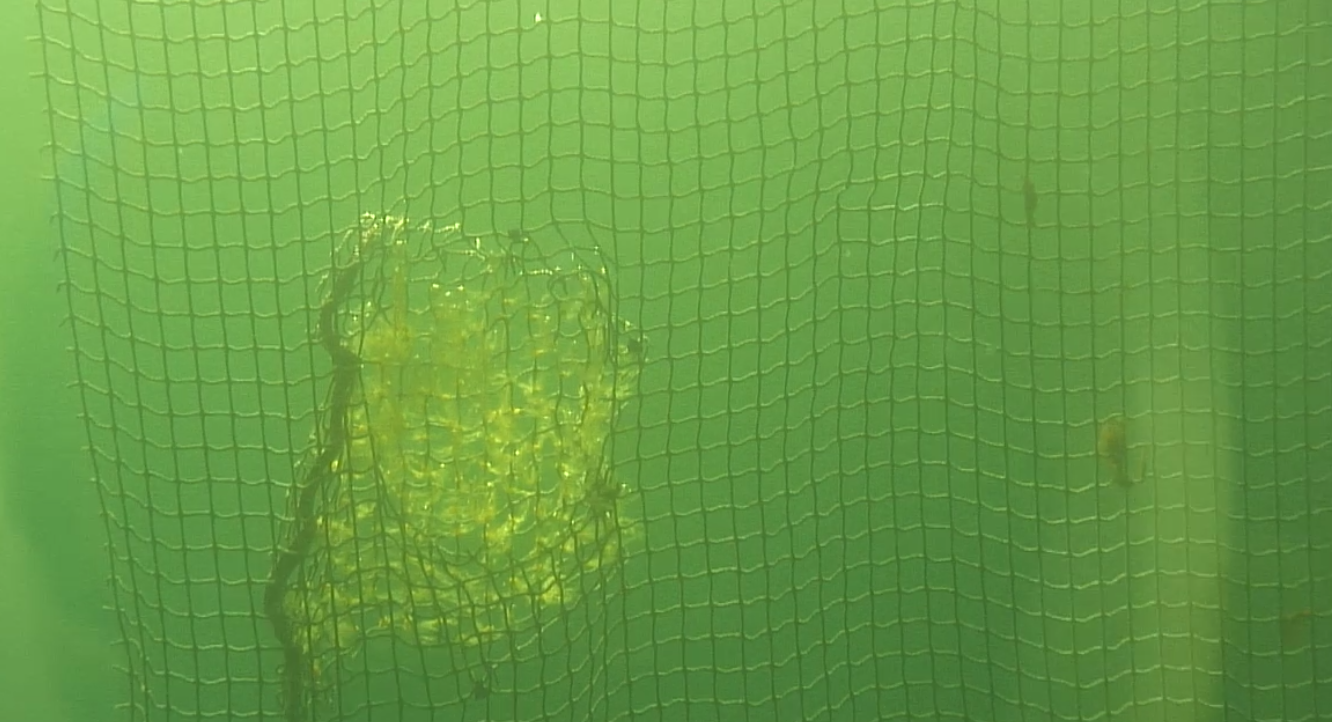
\includegraphics[width=\textwidth]{video_zoom_2}
	\caption{View of masks in and growth simulation on net at \SI{1.5}{\metre}.}
	\label{fig:video_zoom_2}
\end{figure}

\begin{figure}[htbp]
	\centering
	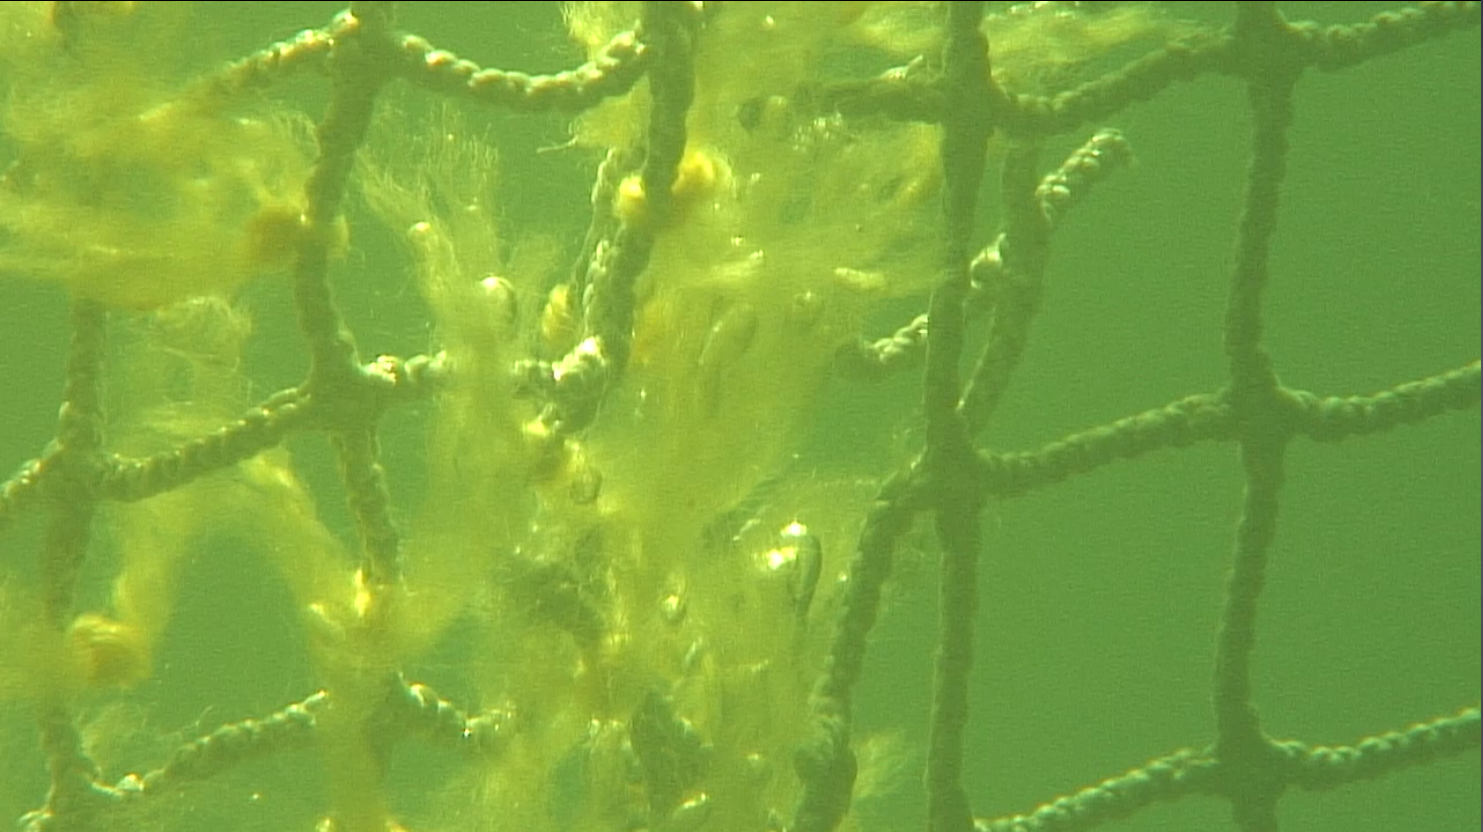
\includegraphics[width=\textwidth]{video_zoom_1}
	\caption{Same view as in figure \ref{fig:video_zoom_2}, but using the optical zoom in the camera.}
	\label{fig:video_zoom_1}
\end{figure}



Another problem with the video stream that were discovered at a later stage, is how the camera behaves during rapid movement. 
Due to the perceived low light conditions, it seems that the camera increases the shutter speed to allow more 
light into the camera sensor. 

The shutter speed of the camera during the underwater operation seems to 
have been \SI{1/50}{\second} which caused motion blurring to be introduced. This 
causes the masks in the net to be blurred out, resembling that of a 
Gaussian filter. Back in the office, it was discovered that the camera can lock the 
shutter in different modes, allowing manual control of the shutter. The camera 
is capable of a speed of \SI{1/2}{\second} to \SI{1/10000}{\second} in 21 steps. 
The movement artefacts can be seen in figure \ref{fig:fart_ufok}.


\begin{figure}[hbp]
	\centering
	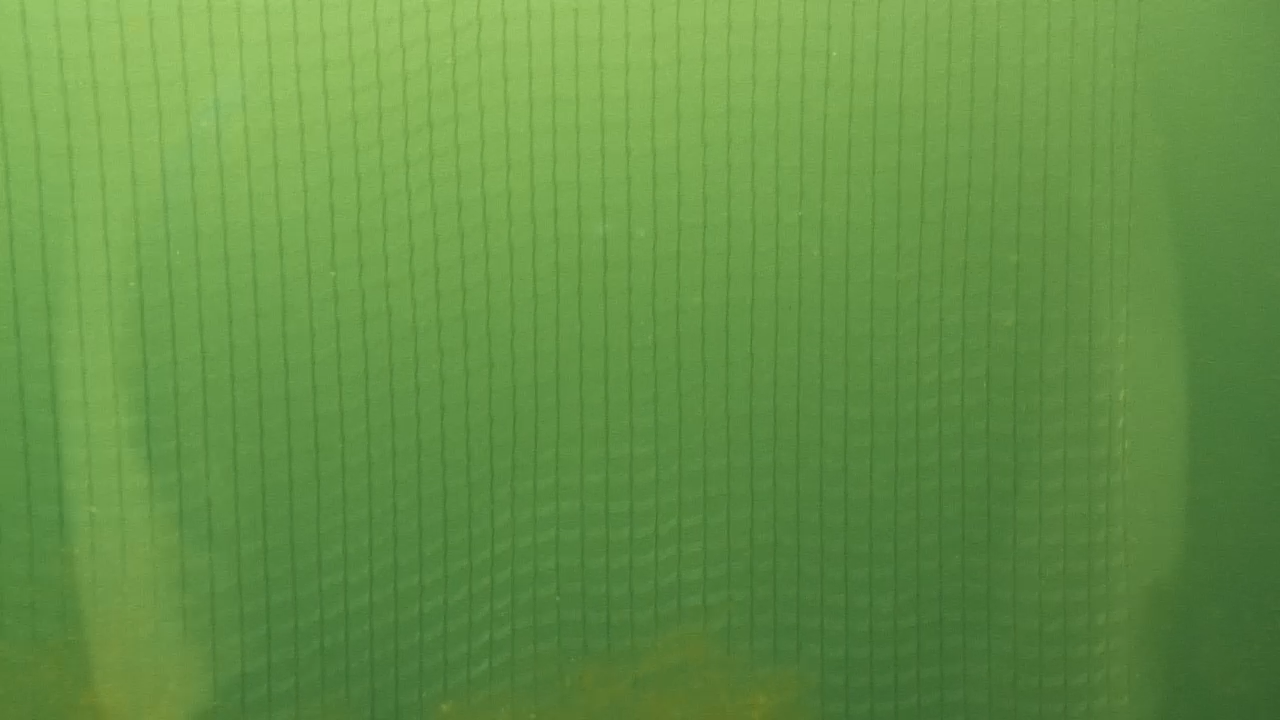
\includegraphics[width=\textwidth]{fart_ufok}
	\caption{The raw video during rapid movement}
	\label{fig:fart_ufok}
\end{figure}


\section{Software}
The software used during the field tests were mainly the software provided with the Ultrastudio unit. This capture software provided a stable connection to 
the Ultrastudio unit. It also made it possible to capture all the sequences that were done as raw video. The raw video could then be compressed on a later 
stage to ensure that the quality during tests were as close to the raw stream as possible.

\subsection{Capture constraints}

During the initial tests, it was discovered that the throughput of the capture was far greater than that the laptop were able 
to save to disk. This meant that the capture were done to ram, and push to the disk at a later stage. This meant that the length of each sequence needed to 
be quite short, as the laptop that were used would exhaust its memory in approximately 30 seconds of capture. This caused frames to 
be skipped in some of the captured files.